\documentclass[english]{article}
\usepackage[T1]{fontenc}
\usepackage[latin9]{inputenc}
\usepackage[active]{srcltx}
\usepackage{float}
\usepackage{graphicx}
\usepackage{babel}
\begin{document}



\section{Introduction}

\begin{figure}[H]
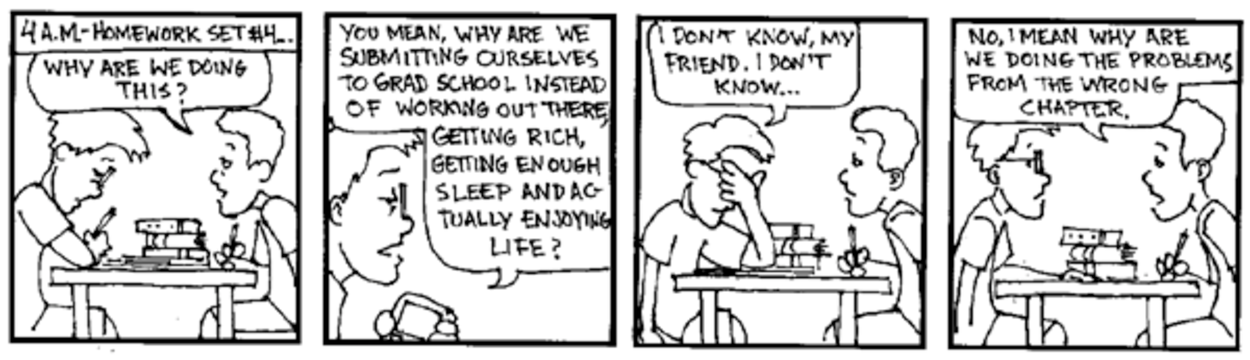
\includegraphics[scale=0.5]{Desktop/cos424_project/Report/phd1029}
\end{figure}


The above comic is one of the most popular comics in the PhD comics
website, which is maintained by PhD students and very popular among
them, and ironically raises the important question of what are the
level of students' satisfaction on different graduate (PhD) programs.
However, when a prospective graduate student is trying to choose a
PhD program, the current tools available for searching for this information
are quite limited. Sites such as usnews.com and forbes.com offer little
if any information on student satisfaction, while less formal ranking
systems such as collegeprowler.com (now moved to colleges.niche.com)
have sparse data and suffer from the bias problems inherent in any
crowd sourced review system. Thus, in this project we tried to address
the lack of information on this question. We used a completely different
approach to the problem: we applied machine learning techniques to
a text corpus consisting of dissertation acknowledgment sections from
different universities. 

More specifically, we used sentiment analysis on the acknowledgment
sections of submitted PhD theses to ranking US universities based
on how satisfied students were which their PhD when they finished
it. We believe that the dissertation acknowledgment session of a PhD
thesis has features that correlate with student satisfaction. For
instance, universities with longer and more positive acknowledgments
likely have more satisfied PhD student than universities with more
terse ones.

Our approach has important advantages when compared to other approaches
currently available. For instance, acknowledgment sessions tend to
have an open format and be straight forward, thus they provide a good
target for successful sentiment analysis and a measure of satisfaction
that is less sensitive to questionnaire biases. Moreover, we have
a much larger sample size than other methods addressing PhD students
satisfaction, as we collected about 2000 acknowlegment sessions, which
was a subset of the 3.6 million english PhD theses listed on \textbackslash{}verb|proquest.com|,
for our analyses.
\end{document}
